\chapterimage{bdiseno.jpg}
\chapter{Diseño}
\begin{figure}[H]
	\centering
	
\includegraphics[width=1\linewidth]{diseno}
    \centering
\end{figure}
\section{Introducción}

El diseño del software, constituye una de las bases más importantes a la hora de crear nuevos sistemas. Hoy en día la complejidad creciente del software hace que el riesgo de construir sistemas que no alcancen los objetivos sea muy alto. Para evitar ese riesgo conviene construirlo a partir de una buena fase de planificación mediante diagramas UML que permitan cumplir las expectativas tanto del desarrollador como las del cliente. A continuación se presentarán algunos de los diagramas más importantes relacionados con el diseño del sistema de gestión de monitorías.

\newpage

\section{Diagrama de Clases de Análisis}

Los diagramas de clases de análisis facilitan la realización de los casos de uso del sistema y sirve como una simplificación del modelo de diseño. Entre los 3 elementos que se visualizan en estos diagramas se encuentran la Interfaz, qué es una clase estereotipada la cual describe la realización de los casos de uso del sistema. El otro elemento es el controlador, donde se plasma la lógica del negocio y el último elemento es la entidad, donde se encuentra la persistencia del sistema. 

A continuación se muestra el diagrama de clases de análisis para la parte de la autenticación del usuario.
\begin{figure}[H]
	\centering
	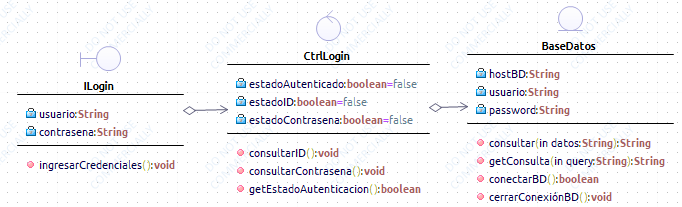
\includegraphics[width=1\linewidth]{dcaLogin}
	\centering
	\caption{Diagrama de Clases de análisis para el Login de la plataforma.}
	\label{fig:dClaALogin}
\end{figure}

Por otro lado se tiene para la certificación de monitorías el siguiente diagrama:

\begin{figure}[H]
	\centering
	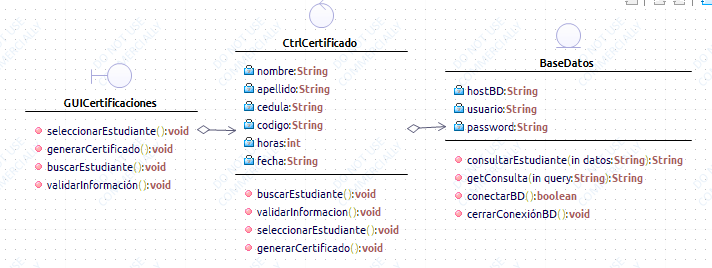
\includegraphics[width=1\linewidth]{dcaCertificacion}
	\centering
	\caption{Diagrama de Clases de análisis para la certificación de monitoría.}
	\label{fig:dcaCertificacion}
\end{figure}
\clearpage
La siguiente figura representa el diagrama de clases de análisis de el contacto entre monitor y profesor

\begin{figure}[H]
	\centering
	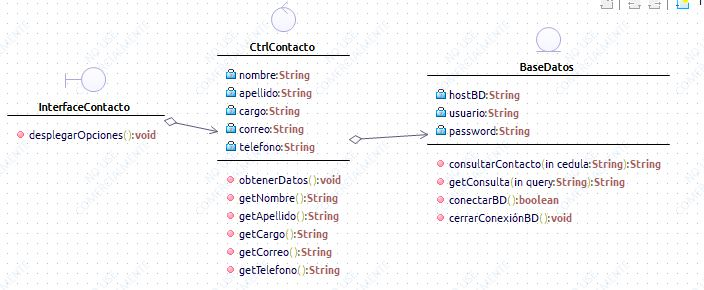
\includegraphics[width=1\linewidth]{dcaContacto}
	\centering
	\caption{Diagrama de Clases de análisis para el contacto Docente-Monitor.}
	\label{fig:dcaContacto}
\end{figure}

En el próximo diagrama de clases de análisis se puede observar las clases que interfieren en el proceso de publicar clasificados.

\begin{figure}[H]
	\centering
	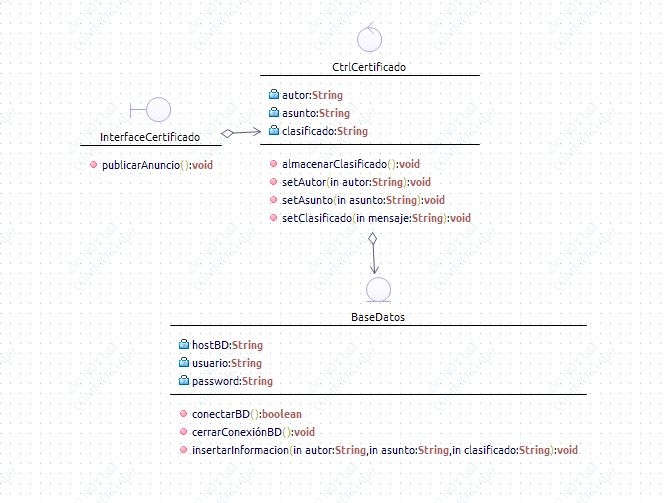
\includegraphics[width=1\linewidth]{dcaClasificados}
	\centering
	\caption{Diagrama de Clases de análisis para el proceso de publicar clasificados .}
	\label{fig:dcaClasificado}
\end{figure}
\clearpage
Por último se tiene el diagrama de clases de análisis de la certificación de las horas de las monitorías.

\begin{figure}[H]
	\centering
	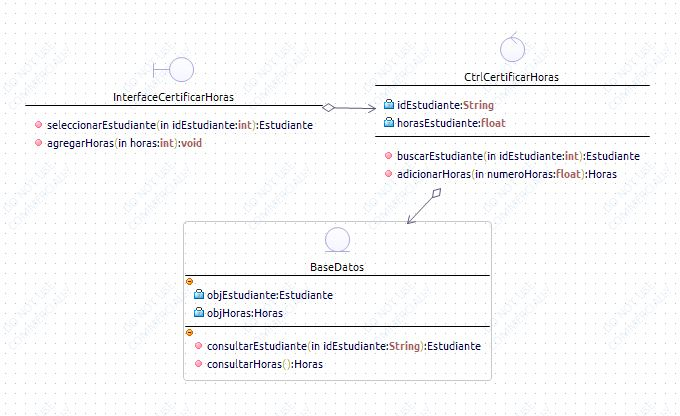
\includegraphics[width=1\linewidth]{dcaCertificarHoras}
	\centering
	\caption{Diagrama de Clases de análisis para el proceso de certificación de horas.}
	\label{fig:dcaCertificarHoras}
\end{figure}

\newpage

\section{Diagrama de Clases}

Un diagrama de clases describe los tipos de objetos que hay en el sistema y las diversas clases de relaciones estáticas que existen entre ellos.
Es importante identificar las relaciones entre las clases. El nombre de la asociación debe dejar claro que una entidad utiliza a otra clase como parte de sus atributos o características. Se debe tener en cuenta que entre dos clases puede existir más de una relación.\cite{Sergio_2015}
\newline
De acuerdo a los diagramas de secuencia y objetos, se realizó una construcción de los diagramas de clase de acuerdo con la utilidad que tiene coloso, a partir de las clases generadas se procedió a editar cada una de estas clases, agregando una serie de atributos y métodos que en un principio se consideran necesario.

El primer diagrama consiste en las clases que administran la forma de ingresar a la plataforma:

\begin{figure}[H]
	\centering
	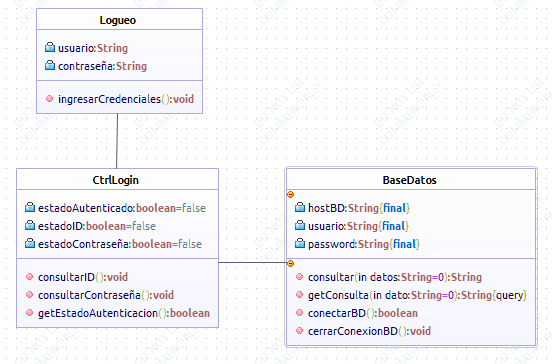
\includegraphics[width=0.8\linewidth]{dclogin}
    \centering
    \caption{Diagrama de Clases para el Login de la plataforma.}
	\label{fig:dClaLogin}
\end{figure}

\newpage
Ahora, en la siguiente imágen se muestra el diagrama de clases para la generación de certificados, en este diagrama la clase control depende de la clase de base de datos para ejecutar su lógica y ésta a su vez usa de una interfaz gráfica donde el usuario interactúa con el aplicativo y este visualiza los datos entregados.

\begin{figure}[H]
	\centering
	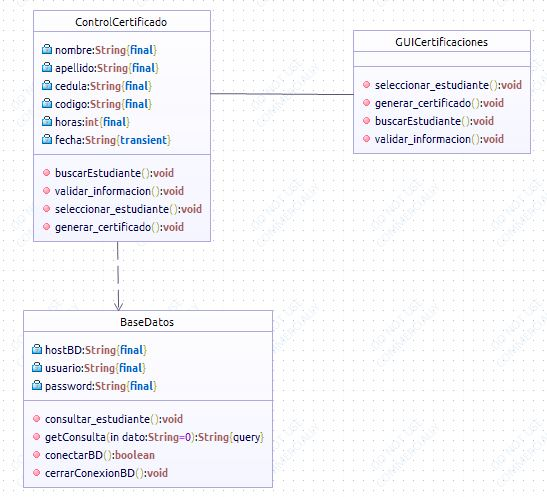
\includegraphics[width=0.8\linewidth]{DiagramaClases}
    \centering
    \caption{Diagrama de Clases para la generación de certificados monitoria.}
	\label{fig:dClaCertificado}
\end{figure}

\newpage
Manera similar sucede con el diagrama de clases para la visualización de contactos, cuya finalidad es obtener unicamente los datos de contacto de los usuarios.
\begin{figure}[H]
	\centering
	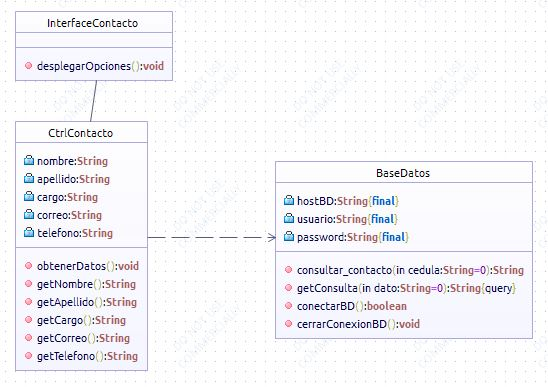
\includegraphics[width=1\linewidth]{dcContacto}
    \centering
    \caption{Diagrama de clases para la visualización de contactos.}
	\label{fig:dClaContacto}
\end{figure}
\newpage
\clearpage
Uno de los beneficios que ofrece la plataforma de gestión de monitorías es el uso de clasificados por parte de los profesores para completar las horas requeridas por el monitor, en base al diagrama de secuencia de la figura 3.7 se propone el siguiente diagrama de clases:

\begin{figure}[H]
	\centering
	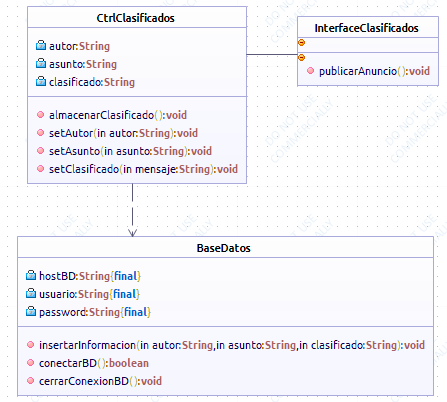
\includegraphics[width=0.8\linewidth]{dcClasificado}
    \centering
    \caption{Diagrama de clases para la publicación de clasificados}
	\label{fig:dClaClasificado}
\end{figure}
\clearpage
La certificación de las horas de monitoria es uno de los procesos imprscindibles en el desarrollo del proyecto, puesto que con este se busca aportar al cumplimiento de varios requerimientos, como los de eliminar el papeleo y facilitar el proceso de certificación, por lo que es importante hacer una correcta espicificación de este.
\begin{figure}[H]
	\centering
	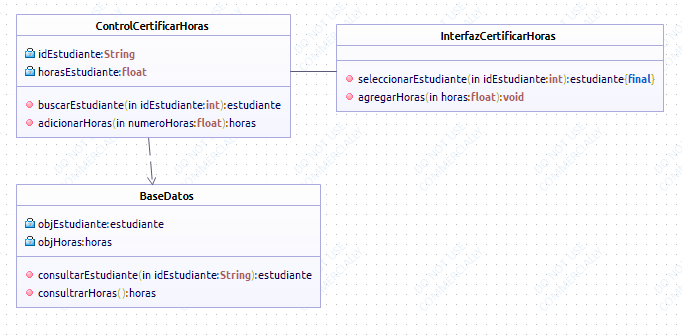
\includegraphics[width=1\linewidth]{dcCertifi}
    \centering
    \caption{Diagrama de clases para la certificación de horas de monitoría}
	\label{fig:dClaCertifi}
\end{figure}

\section{Diagrama de Objetos}

\newpage

\section{Diagrama de Estructura Compuesta}

\newpage

\section{Patrones}
Según Gamma en su libro Patrones de Diseño, define a un patrón de diseño como una descripción
de clases y objetos comunicándose
entre sí adaptada para resolver un
problema de diseño general en un
contexto particular. Con los patrones de diseño es posible saber cual fue la intencionalidad con la que se desarrolló una aplicación y cual será a futuro la intención con la que se desarrolla en el presente. El patrón de diseño no es sólo una plantilla para reusar; es todo un idioma de diseño que estandariza la forma de diseñar aplicaciones, garantizando su fácil evolución, prueba y mantenimiento\cite{Bol_2014}.

Existen 3 tipos de patrones:
\begin{itemize}
\item Creacionales: 
\item Estructurales
\item De comportamiento
\end{itemize}
\subsection{Patrones creacionales}
Los patrones creacionales proporcionan ayuda a la hora de crear instancias de objetos. El objetivo
de este tipo de patrones es el de abstraer el proceso de instanciación y ocultar los detalles de cómo los objetos
son creados o inicializados \cite{Bol_2014}.
Dentro de los patrones creacionales se pueden encontrar los siguientes:
\begin{enumerate}
\item Método Fábrica
\item Fábrica Abstracta
\item Prototype
\item Constructor
\item Singleton
\end{enumerate}

Para el caso concreto de nuestro proyecto, se hará uso del patrón creacional singletón. Por lo que sólo se hará énfasis profundo en éste patrón.
\newpage
\paragraph{Singleton}
El patrón Singleton, también conocido como instancia única, nos permite tener un controlar en número de instancias de un objeto, en este caso, como su nombre lo indica, defina la creación de una única instancia.
\newline
\indent\textbf{Estructura}
\newline
\begin{figure}[H]
	\centering
	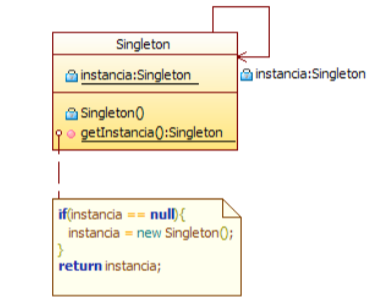
\includegraphics[width=0.5\linewidth]{estructuraSingleton}
    \centering
    \caption{Estructura del patrón Singleton.}
	\label{fig:eSingleton}
\end{figure}
\indent\textbf{Caso de estudio}
\newline
\begin{figure}[H]
	\centering
	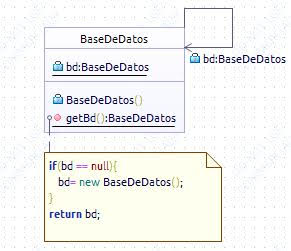
\includegraphics[width=0.5\linewidth]{singleton}
    \centering
    \caption{Singleton del sistema de gestión tutoríaas.}
	\label{fig:singleton}
\end{figure}

\indent Dentro del diseño del aplicativo es necesario garantizar que la base de datos de la que se hace uso sea la misma en todo el aplicativo y que no se creen multiples instancias de esta, por lo que se hará uso del patrón de diseño Singleton para garantizar una única instancia de la base de datos y que esta sea utilizada en todo el aplicativo. Podrá observar un ejemplo de su implementación en el anexo 8.1.1.
\newpage
\subsection{Patrones Estructurales}
Los patrones estructurales se enfocan en como las clases y objetos se componen para formar
estructuras mayores, los patrones estructurales describen como las estructuras compuestas por clases
crecen para crear nuevas funcionalidades de manera de agregar a la estructura flexibilidad y que la
misma pueda cambiar en tiempo de ejecución lo cual es imposible con una composición de clases
estáticas\cite{estruct}.
Dentro de los patrones estructurales se pueden encontrar los siguientes:
\begin{enumerate}
\item Puente
\item Adaptador
\item Componente
\item Decorador
\item Fachada
\item Peso Ligero
\item Proxy
\end{enumerate}

Para el caso concreto de nuestro proyecto, se hará uso de los patrones estructurales Componente, Fachada y Proxy. Por lo que sólo se hará énfasis profundo en estos patrones.
\paragraph{Patrón Fachada}
\indent El patrón fachada provee una interface unificada para un conjunto de interfaces en un subsistema, la fachada es una interface de alto nivel que facilita el uso de un subsistema. Su uso principal consiste en la posibilidad de crear un sistema de niveles\cite{Bol_2014}.
\newline
\indent\textbf{Estructura}
\newline
\begin{figure}[H]
	\centering
	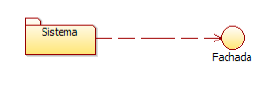
\includegraphics[width=0.5\linewidth]{fachada}
    \centering
    \caption{Estructura del patrón fachada.}
	\label{fig:eFachada}
\end{figure}
\indent\textbf{Caso de estudio}
\begin{figure}[H]
	\centering
	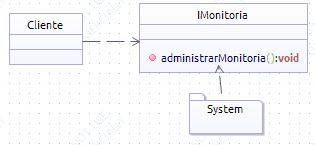
\includegraphics[width=0.5\linewidth]{dcFachada}
    \centering
    \caption{Fachada del sistema de gestión de tutorías.}
	\label{fig:dcFachada}
\end{figure}
\indent Para el diseño del aplicativo de gestión de monitorías se utilizará una fachada que reuna las implementaciones más fundamentales con las que el usuario interactuará. Desacoplando la implementación del cliente con todo el subsistema y simplificando su uso. Puede observar un ejemplo de su implementación en el Anexo 8.1.2.
\newpage
\paragraph{Patrón Componente}
El patrón componente simplifica el uso de varios objetos similares organizandolos en una estructura tipo árbol que representa el todo-parte\cite{Bol_2014}, lo cual simplifica la creación de algoritmos y objetos complejos haciendo uso de la recursión al tratar al todo igual que a una parte.
\begin{figure}[H]
	\centering
	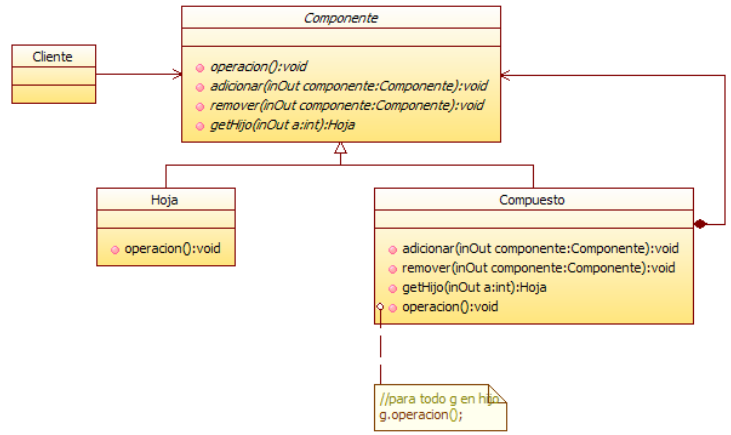
\includegraphics[width=0.8\linewidth]{PatronComponente}
    \centering
    \caption{Estructura del patrón componente.}
	\label{fig:eComponente}
\end{figure}
\indent\textbf{Caso de estudio}
\newline
\begin{figure}[H]
	\centering
	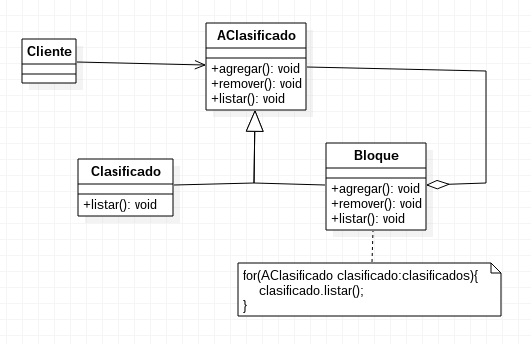
\includegraphics[width=0.6\linewidth]{composite}
    \centering
    \caption{Patrón componente del sistema de gestión de tutorías..}
	\label{fig:composite}
\end{figure}
\indent Dentro de la aplicación de monitorias se creará una zona de clasificados en donde los monitores podrán observar las publicaciones hechas por los profesores que requieran de sus servicios. Para el manejo de estos clasificados se ha decidido hacer uso del patrón componente, el cual permite agrupar los clasificados en una estructura en forma de árbol, lo que permite hacer uso de la recursión para facilitar la forma en la que se van a visualizar los clasificados. Podrá observar un ejemplo de su implementación en el anexo 8.1.3. 
\newpage
\paragraph{Patrón Proxy}
Provee un sustituto o marcador para otro objeto que controla el acceso a él. Controla el acceso a un objeto o lo representa localmente o por su alta demanda.\cite{Bol_2014}.
\newline
\indent\textbf{Estructura}
\newline
\begin{figure}[H]
	\centering
	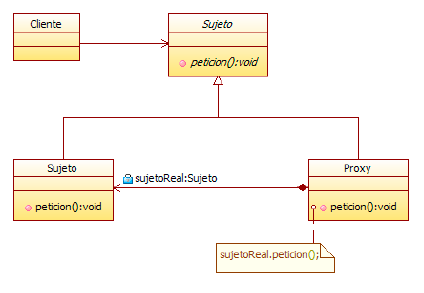
\includegraphics[width=0.5\linewidth]{proxyestruct}
    \centering
    \caption{Estructura del patrón proxy.}
	\label{fig:eProxy}
\end{figure}
\indent\textbf{Caso de estudio}
\begin{figure}[H]
	\centering
	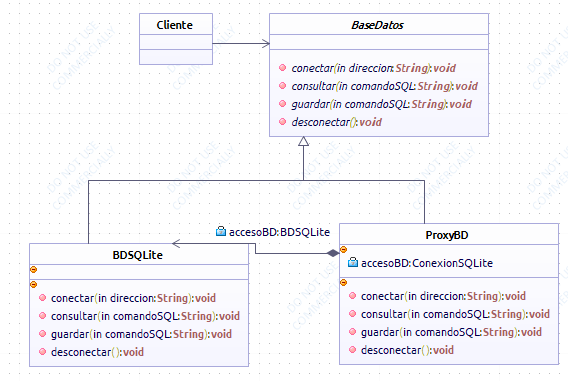
\includegraphics[width=0.5\linewidth]{dcProxy}
    \centering
    \caption{Implementación del patrón proxy.}
	\label{fig:dcProxy}
\end{figure}
\indent El patrón Proxy actúa en el diseño del sistema de gestión de monitorías como intermediario para poder realizar operaciones en la base de datos SQLite, el proxy recibe la solicitud de alguna operación en la base de datos, y si es posible hacerla se delegan las funciones a la clase BDSQLite, caso contrario no se ejecuta ninguna acción lo cual reduce el uso de recursos. Podrá observar un ejemplo de su implementación en el anexo 8.1.4.
\newpage
\subsection{Patrones de Comportamiento}
Los patrones de comportamiento explican la forma en la que los objetos interactúan entre sí. Describe como los diferentes objetos y clases intercambian mensajes entre ellos para hacer que las cosas funcionen y describir como los pasos de una tarea en específico es dividida a lo largo de distintos objetos. A diferencia de los patrones creacionales que solo describen el momento en que se crean los objetos y los patrones estructurales que describen una estructura más o menos estática, los patrones de comportamiento describen un proceso o flujo de información\cite{behavioral}.
Dentro de los patrones de comportamiento se pueden encontrar los siguientes:
\begin{enumerate}
\item Cadena de Responsabilidad
\item Comando
\item Interprete
\item Iterador
\item Mediador
\item Momento
\item Observador
\item Estado
\item Estrategia
\item Método Plantilla
\item Visitador
\end{enumerate}

Para el caso concreto de nuestro proyecto, se hará uso del patrón de comportamiento comando. Por lo que sólo se hará énfasis profundo en éste patrón.
\paragraph{Patrón Comando}
El patrón comando nos permite encapsular una petición en un objeto, es decir que nos permite parametrizar a los clientes con diferentes peticiones, esto significa que podemos hacer peticiones a objetos de nuestra aplicación sin ser especificados, este es un método importante, debido a que como desarrolladores muchas veces no tenemos modo de conocer al receptor de la petición, ni de saber que operaciones se efectuaran, en términos conceptuales este patrón nos permite asegurar el encapsulamiento y por ende la seguridad de nuestra información
\newline
\indent\textbf{Estructura}
\begin{figure}[H]
	\centering
	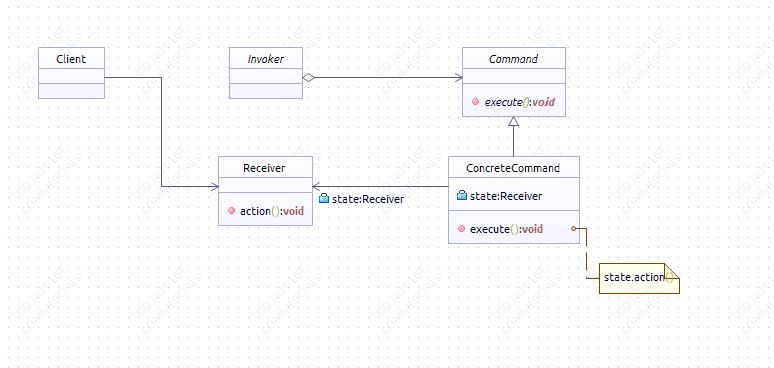
\includegraphics[width=0.8\linewidth]{mComando}
    \centering
    \caption{Estructura general del patron comando.}
	\label{fig:mComando}
\end{figure}
\clearpage
\indent\textbf{Caso de estudio}
\begin{figure}[H]
	\centering
	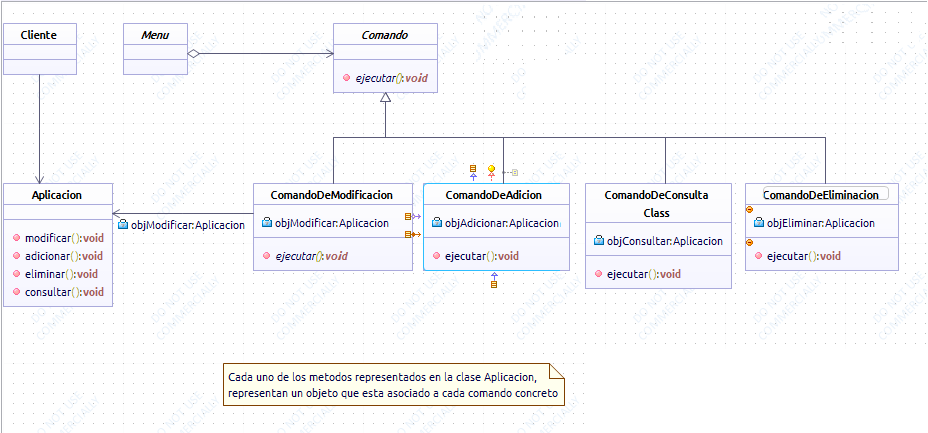
\includegraphics[width=0.6\linewidth]{ceComando}
    \centering
    \caption{Comando del sistema de gestión de tutorías.}
	\label{fig:ceComando}
\end{figure}
\indent La clave de este patrón es la clase abstracta Comando, esta declara una interfaz para ejecutar las líneas de operaciones, en este caso, esta clase tiene consigo una operación, también abstracta la cual se le suele llamar Ejecutar, con ello las subclases de orden, especifican un receptor-acción (en nuestro caso el receptor seria nuestra aplicación, por el otro lado la acción seria el comando) guardando el receptor como una variable de instancia e implementado, mientras que Ejecutar se usa para invocar la petición. Por ende, el receptor debe poseer el conocimiento necesario para llevar a cabo la petición. Una de las características y principales, y quizá la que nos da una conveniente ventaja es la de tener la posibilidad de deshacer las operaciones realizadas, también y por obvias razones buscamos independizar el momento de la petición del momento de la ejecución.
\newline

Como ya habíamos mencionado, al tener nuestra clase comando, debemos tener la especificación, es decir la clase concreta de nuestro comando, con ello nos permitimos separar tareas, y es esta clase la que conocerá la procedencia de la petición.  La clase menu será nuestra interfaz gráfica, es decir un menú con opciones desplegables sobre ciertas tareas a cumplir.Y por otro lado la clase app será la que implemente la funcionalidad real, es decir nuestra aplicación en sí, esta sera nuestra clase receptor. Podrá observar un ejemplo de su implementación en el anexo 8.1.5.
\newpage
